\documentclass[10pt,letter]{article}

\usepackage{fullpage}
\usepackage{setspace}
\usepackage{parskip}
\usepackage{titlesec}
\usepackage{xcolor}
\usepackage{lineno}






\PassOptionsToPackage{hyphens}{url}
\usepackage[colorlinks = true,
            linkcolor = blue,
            urlcolor  = blue,
            citecolor = blue,
            anchorcolor = blue]{hyperref}


\usepackage[round]{natbib}
\let\cite\citep

%\usepackage{eso-pic}
%\AddToShipoutPictureBG{\AtPageLowerLeft{\includegraphics[scale=0.7]{powered-by-Authorea-watermark.png}}}

\renewenvironment{abstract}
  {{\bfseries\noindent{\large\abstractname}\par\nobreak}}
  {}

\renewenvironment{quote}
  {\begin{tabular}{|p{13cm}}}
  {\end{tabular}}

\titlespacing{\section}{0pt}{*3}{*1}
\titlespacing{\subsection}{0pt}{*2}{*0.5}
\titlespacing{\subsubsection}{0pt}{*1.5}{0pt}


\usepackage{authblk}
\makeatletter
\renewcommand\AB@authnote[1]{\rlap{\textsuperscript{\normalfont#1}}}
\renewcommand\Authsep{,~\,}
\renewcommand\Authands{,~\,and }
\makeatother


\usepackage{graphicx}
\usepackage[space]{grffile}
\usepackage{latexsym}
\usepackage{textcomp}
\usepackage{longtable}
\usepackage{multirow,booktabs}
\usepackage{amsfonts,amsmath,amssymb}
\providecommand\citet{\cite}
\providecommand\citep{\cite}
\providecommand\citealt{\cite}
% You can conditionalize code for latexml or normal latex using this.
\newif\iflatexml\latexmlfalse
\DeclareGraphicsExtensions{.pdf,.PDF,.png,.PNG,.jpg,.JPG,.jpeg,.JPEG}

\usepackage[utf8]{inputenc}
\usepackage[ngerman,english]{babel}



\begin{document}

\title{Unnamed Article}



\author[ ]{jonjunduan}%
\affil[ ]{Affiliation not available}%




\vspace{-1em}



  \date{\today}


\begingroup
\let\center\flushleft
\let\endcenter\endflushleft
\maketitle
\endgroup







\section{Research Context }\label{research-context}

The goal of the current research is to understand the economic
consequences of integrating renewable energy into existing power
systems, design policies to achieve an optimal mix of generating assets
in an electricity grid, and determine the costs and benefits of using
renewable energy sources to reduce carbon dioxide and other greenhouse
gas (hereafter just CO\textsubscript{2}) emissions.

In most countries, electricity and heat constitute the most important
sector accounting for CO\textsubscript{2} emissions, although this
sector ranks lower in Canada, because 59\% of its electricity comes from
hydro sources. Yet, 35 coal power units across Canada, mainly in
Alberta, Saskatchewan, Manitoba, New Brunswick and Nova Scotia,
represent over 70\% of emissions in Canada's electricity sector, while
providing only 11\% of the country's electricity (David Suzuki
Foundation. 2016). The importance of coal-fired power globally cannot be
overemphasized -- about 80\% of China's and more than two-thirds of
Australia's and India's power is generated by coal, while more than 40\%
of electricity produced in the United States and Germany comes from
coal.\footnote{http://\href{http://wdi.worldbank.org/table/3.7\%20accessed\%20September\%2018}{wdi.worldbank.org/table/3.7}
  {[}accessed April 4, 2017{]}}

To mitigate the impact of coal on climate change, many developed
countries are planning to phase out coal-fired power plants. To our best
knowledge, Austria, Britain, Denmark, Finland, France, the Netherlands
and Canada have committed to close coal-fired plants by 2025 or 2030
(McCarthy 2016). However, to meet the growing demand for electricity,
more than 570 GW of coal-fired power capacity was under construction
globally as of January 2017.\footnote{Construction of new coal-fired
  power plants fell worldwide in 2016, EnergyMarketPrice,
  \url{http://www.energymarketprice.com/energy-news/construction-of-new-coal-fired-power-plants-fell-worldwide-in-2016}
  {[}accessed April 4, 2017{]}} Although well below last year, this
represents 570 new 1,000 MW capacity new plants, and does not include
those recently approved or planned (Guo 2017). China, India and other
developing countries, and even rich countries like Japan, are building
or planning to build new coal power stations.

It is not easy for us to get rid of coal. In 2012, with regulations on
emissions from the coal-fired electricity sector, Canada became the
first major coal user to ban construction of traditional coal-fired
power stations.\footnote{In 2012, the Canadian federal government
  approved the Reduction of Carbon Dioxide Emissions from Coal-fired
  Generation of Electricity Regulations. The regulation requires that
  coal-fired generation units meet a GHG emissions intensity target once
  it reaches end of life.} However, without coal power to meet the
growing demand of electricity, Alberta and Saskatchewan had invested on
natural gas power stations, which did little to reduce their total
greenhouse gas emission (Environment Canada 2011).

To stop climate change, we need to move away from fossil fuels, which
requires investment in alternative energy sources. On the pathway to
decarbonization, many people put a lot faith on renewables. At the
United Nations Climate Change Conference, nearly 50 countries agreed to
make their energy production 100 percent renewable by 2050 (Payton
2016). In Canada, Alberta's government plans to phase out all coal-fired
electricity generation facilities by 2030, and replace two-thirds of the
lost electricity production by renewables (Alberta Government 2012).

Decarbonization comes with a cost. First at all, even if costs are
falling over time, most renewables, such as wind and solar, are still
more expensive than the fossil fuels (Lazard 2016). Replacing fossil
fuels by renewables means rising electricity bills. Moreover, a
stumbling block in the development of modern renewable energy globally
is the intermittent nature of renewable energy, and of solar and wind
power specifically. Because of its intermittency, wind and solar cannot
be considered reliable as either baseload sources of electricity or
suitable for addressing peak demand (van Kooten et al. 2016), and thus
the integration of renewable energy into the grid has proven problematic
for many countries (Timilsina et al. 2013). From 2015, Hawaii local
utility company has slowed down connection of new rooftop solar system
to the grid due to the safety and reliability issue of the grid.
Intermittency in wind (and solar) power output is unavoidable, and the
gaps result in large costs of ramping existing generating assets or
investing in new assets to compensate for this intermittency (van Kooten
2016a). Therefore, the opportunity cost of introducing renewables is
much higher than the explicit accounting cost.

To balance the trade-off between clean and cheap electricity, certain
public policies are needed to provide incentives for firms to develop
and operate renewable generating assets.\footnote{In 2016, after the
  Nevada Public Utilities Commission lowered the price that utility
  companies pay homeowners for their electricity from rooftop solar
  panels, the solar installations in Nevada decreased dramatically.
  http://www.pbs.org/newshour/bb/debate-over-solar-rates-simmers-in-the-nevada-desert/
  {[}accessed April 4, 2017{]}} On October 3, 2016, the Canadian federal
government announced that, unless provinces were more aggressive in
their policies to reduce CO\textsubscript{2} emissions, it would
implement a carbon tax that would start at \$10 per tonne of carbon
dioxide (tCO\textsubscript{2}) beginning in 2017 and increase annually
by \$10/tCO\textsubscript{2} until it reached \$50/tCO\textsubscript{2}
in 2021. Meanwhile, Ontario adopted a cap-and-trade system for
facilities producing over 25,000 tCO\textsubscript{2} annually (Ontario
Power Authority 2016), while providing a feed-in tariff (FIT) for
medium- and small-scale renewable energy providers, known as microFIT,
and renewable procurement processes for large renewable energy providers
(IESO 2016). Furthermore, the Alberta government implemented an
economy-wide carbon tax of \$20/tCO\textsubscript{2} beginning in 2017
and increases it to \$30/tCO\textsubscript{2} in 2018; provide subsidies
to encourage renewable energy; and cap emissions from oil sands
developments at 100 megatons of CO\textsubscript{2} (Government of
Alberta 2016).

The current research will study the cost and benefit to society from
replacing fossil fuels by renewables in a power system. To determine
what is the optimal generation mix in a carbon constrained jurisdiction
such as Alberta, we adopt a grid optimization model to solve this
problem (van Kooten et al. 2013). With the assumptions of rational
expectation of the grid operator/asset owner and interties between
adjacent jurisdictions, the grid operator/asset owner optimize load
across assets in each hour. Using this optimization grid model, we can
calculate the optimal tax or subsidy required to introduce renewables
into grid and to achieve a climate change target. Therefore, we also can
get the estimated social cost or shadow price of the decarbonization
from a fossil-fuel based electricity sector.

Moreover, to examine the performance of a grid, we need accurate
economic cost evaluation for generation technologies. This economic cost
evaluation needs to take explicit and implicit costs into account.
Different technologies are developed to evaluate the social benefits and
costs of electricity. I will look at the impact of the cost of
electricity on the generating mix by using the
load-duration-screening-curve framework, and I will use positive
mathematical programming to calibrate the economic cost of generation
technologies.

\subsection{It is time to change the power
system}\label{it-is-time-to-change-the-power-system}

It is not easy to incorporate renewables into the power system. The
problem is that the original power system is not designed for variable
and distributed power resources like wind and solar energy. To build an
electricity power system that integrates the renewable sources of
energy, we need to redesign the power system by reforming the pricing
mechanism, improving regulations, and changing the business model.
Nonetheless, integrating renewable energy sources into an electricity
grid, whether an existing grid or one that is optimally designed,
results in indirect costs imposed on non-renewable assets, costs that
are often ignored when considering the costs of integrating renewables
into an existing or even new grid structure.\footnote{For the same
  reason, Nevada Energy decided to charge rooftop solar panel owners
  more than non-solar users.
  https://www.bloomberg.com/features/2016-solar-power-buffett-vs-musk/
  {[}accessed April 4, 2017{]}}

There are at least two challenges we face when we incorporate renewables
into the power system. One is the intermittency of renewables. The wind
is not always blowing and the sun is not always shining. They are not
dispatchable like gas or coal power. When we need power, we can push the
throttle to increase power output or quickly start another gas
generation unit, but we cannot make the wind blow. In the beginning of
2017, the South Australian blackout was blamed on wind generation
failures (Murphy et al. 2017). We still rely on other controllable power
sources as backup to provide reliable energy supply.

The second challenge is that wind and solar power disrupt electricity
systems. Under the current power system, wind and solar energy have
almost zero marginal production cost, so in the bidding competitions
they can drive other generation units out when the wind and solar are
available. The return of the other conventional generation assets will
decline and, in the long run, the investment of those conventional
assets will decline.\footnote{Wind and solar power are disrupting
  electricity systems, Economist,
  http://www.economist.com/news/leaders/21717371-thats-no-reason-governments-stop-supporting-them-wind-and-solar-power-are-disrupting
  {[}accessed April 4, 2017{]}} Without those assets as a backup
reserve, when wind or solar was not available, disruptions and blackouts
can occur. Apparently, the current power systems are not ready to
balance the contributions from conventional energy and renewables.

\subsection{The approaches we can
take}\label{the-approaches-we-can-take}

To overcome the intermittency problem of renewables, three approaches
are possible. The first is on the supply side: We can expand the power
grid's connectivity. By locating wind and solar sources of renewable
energy across a large landscape, intermittency can be alleviated to some
extent, depending upon the correlations among wind and solar. In one
place, the wind may stop blowing, but it might start to blow in other
places. Therefore, entrepreneurs in China, South Korea, Russia and Japan
have signed a Memorandum of Understanding that seeks to create the Asia
Super Grid (Hanley 2016). In the same way, it might be possible to
connect European and African grids, or construct a North American power
pool that is connected by much more transmission interties than now
exist. In many cases, however, such huge interconnection projects are
unrealistic from a political and even physical standpoint, and they are
too expensive to undertake. In a much more restricted region, such as
western Canada, the wind power from Alberta and hydro energy from
British Columbia can work together to provide reliable, clean and
sustainable electricity. The current research will study the feasibility
and effect of this small-scale electricity connectivity approach.

One aspect of the BC-Alberta connection relates to the second method for
overcoming intermittency -- storage. Electricity can be stored in the
reservoir behind a hydroelectric dam, in a battery, as compressed air,
or using a chemical storage such as hydrogen. Energy storage is likely
going to play an important role any future power system. The current
research will look at the impact of the hypothetical energy storage in a
carbon constrained province.

The third approach to intermittency occurs on the demand side. With new
technologies, the demand for electricity (known as load) is getting more
forecastable and controllable. Demand side management (load management)
can ``reduce energy consumption, and improve overall electricity usage
efficiency, through the implementation of policies and methods that
control electricity demand'' (Hallberg 2011, p.9). With the development
of new technologies, such as smart grids and net meters, demand response
can make use of ``incentive payments designed to induce lower
electricity use at times of high wholesale market prices or when system
reliability is jeopardized'' (Ibid). The volatility and uncertainty of
the load can be alleviated by better forecasting and other demand-side
management measures. In the future, to better balance the demand and
supply of electricity, we will likely see demand-side management become
a core part of the power system.

All those developments will converge in a future power system. In the
conventional system, generation is centralized, transmission is
unidirectional, and distribution is passive. Electricity is generated in
one place and is transmitted from upstream to downstream. All power
generated must be distributed instantaneously to users (Bakke 2016). In
the future, with the incorporation of intermittent (variable)
renewables, distributed generators such as the rooftop photovoltaic will
grow, and power flows can be bidirectional between different microgrids.
The distributed generation sources are getting more active based on
smart grid control system. More microgrid systems are needed to manage
various energy sources and coordinate controllable demand loads with
power supply sources.\footnote{The smart gird revolution, Energia16,
  http://www.energia16.com/the-smart-grid-revolution/?lang=en
  {[}accessed April 4, 2017{]}} It is time to reconstruct power systems
to accommodate clean but variable renewables. It creates the
opportunities to expand economy just like a hundred of years ago when
the coal and gas replaced wood to become main energy sources.

\subsection{Research Questions}\label{research-questions}

The current research focuses on three types of questions. The first
relates to the economic impacts of incorporating renewables into an
existing power grid and, thereby, to the costs of reducing greenhouse
emissions. High penetration rates of intermittent power sources have an
impact on system CO\textsubscript{2} emissions; however, reduced
emissions from wind power do not replace emissions from thermal power
plants one-for-one. For example, if a coal-fired power plant needs to
lower output to accommodate wind, this leads to inefficiencies in fuel
use resulting from operating below optimal capacity. The first part of
the current research will look at the optimal generation mix, in which a
carbon tax or a feed-in-tariff is used to incentivize removals of fossil
fuel generation and investment in solar panels and wind turbines.

The second part of the current research examines the effect of flexible
storage of electricity on a power system with wind and solar sources.
Storage can alleviate the volatility and uncertainty of renewables, and
also enable coal plants to operate more efficiently, thereby saving fuel
and potentially reducing CO\textsubscript{2} emissions. The connectivity
between different jurisdictions can achieve the same kind of
functionalities. For example, Alberta sells coal-fired power to BC at
night, buying back hydroelectricity at peak times during the day -- de
facto storage. Researchers have investigated the problems associated
with non-dispatchable wind and combined heat and power (CHP) (Liik et
al. 2003; White 2004; Lund 2005). They found that grids are difficult to
manage when the output from large-scale wind farms reaches a maximum
(often at night when CHP output also peaks) and the load is minimal,
while the output from base-load facilities remains high. Unless
electricity can be `dumped' into another jurisdiction during these
times, the adjustment costs imposed on extant generators might be large
(AESO 2008). Successful integration of wind energy depends on the
generating mix of the extant system (Maddaloni et al. 2008b; Prescott \&
van Kooten 2009). The second part of the current research is devoted to
studying a system with massive electricity storage when relatively high
levels of wind and solar generated electricity enter the grid.

The last part of the current research will be devoted to calibration of
electricity cost. Due to the complexity added by integration of
renewables, the costs for generation technologies, especially for wind
and solar, are not so obvious. In the electricity cost literature, many
measures of the levelized costs of electricity (LCOE) are available,
although they often differ because LCOEs are based on estimates of the
overnight construction cost, operating and maintenance costs, fuel
costs, expected capacity factors, and so on. However, the value of
electricity supplies varies over time. In peak time the electricity is
more valuable than in off peak time, which in reflected by the wholesale
market price. Dispatchable generating technologies can be utilized any
time, but intermittent renewables are not so. Relatively, solar power is
more valuable than wind power because solar provides power during the
day time but wind usually provides power during the night. The LCOE
calculations do take into account capacity factors but fail to take into
account the timing of available power from intermittent sources and how
this impacts other assets providing power to the grid at the time
(Joskow 2011).\selectlanguage{ngerman}\footnote{A generating assets capacity capacity factor
  (CF), whether a wind or gas turbine or coal plant, is given by the
  actual megawatt hours (MWh) of electricity generated in one year
  divided by the capacity rating of the asset (MW) multiplied by 8,760
  hours in the year. For example, if a wind turbine has a capacity of
  2.5 MW and generated 3,942 MWh of electricity in a year, it has a CF =
  3942 MWh / (2.5 MW×8760 h) = 0.18, or 18\%.}\selectlanguage{english} To understand the true
economic value of electricity, a comprehensive evaluation should
consider the life time cost and expected profitability of the generating
technologies. Therefore, I will use positive mathematical programming
and maximum entropy methods to calibrate the economic costs for
generation technologies.

By solving a well-calibrated model numerically with real world data, we
can be confident that the model can be used for policy analysis (Paris
2011). We will be able to track changes in the utilization of renewable
power sources and CO\textsubscript{2} emissions as electricity demand
changes over time. We will be able to examine how the optimal structure
of an electricity grid in a particular jurisdiction would change under
various policies to mitigate climate change, highlighting opportunities
for improving the performance of the current electricity system.
Further, we can estimate potential costs of such policies. Finally, we
can determine whether and under what circumstances the grids we examine
can reduce CO\textsubscript{2} emissions by 30\% below 2005 levels by
2030, as has been agreed to in international negotiations (Government of
Canada 2016).

\section{Research Methods }\label{research-methods}

The principal method of analysis will be to develop energy system models
to examine the allocation of power across renewable and non-renewable
generating sources, and between jurisdictions along interties.
Furthermore, the models are used to study the controllable load, demand
response, and distributed generation in the future power system.

My research focus is on western Canada's electricity system and I will
construct a decision support model for two separate electricity grids,
each representing a different mix of generating facilities. The grids
are connected by a transmission intertie that allows the two regions to
trade electricity and meet the constraints imposed by different forms of
generation. (Decision variables include the allocation of generation to
the various generators in the system, plus the capacity of the
transmission line.) One grid relies primarily on hydroelectricity, with
remaining load met by natural gas and other power sources (including
biomass and imported power). The other system meets the base-load power
needs with coal, combined-cycle gas turbine (CCGT) and/or biomass
assets, while marginal power is produced by a mix of hydro and
open-cycle natural gas for peak power production. Renewable sources such
as wind and solar are introduced at various levels. The two grids are
representative of British Columbia and Alberta, respectively; in both
situations, one grid is fossil fuel driven while the `partner' grid
consists almost exclusively of hydro assets. An objective of the
research is to examine how wind investment in Alberta might be able to
employ hydroelectric storage in British Columbia.

The energy system models employ mathematical programming and simulation
methods. The description of the type of models that will be used in the
study is found in van Kooten (2012). The models to be developed in the
proposed research will expand extensively on the prototype modeling to
include the integration of two grids in a more explicit fashion, a
sub-model detailing the operation of hydroelectric facilities, the
interaction between disparate grid operators, the calibration
procedures, and welfare analysis of demand response policies.
% First macro on next line not (yet) supported by LaTeXML: 
% \protect\hypertarget{_Toc478645847}{}{}

\subsection{Mathematical programming}\label{mathematical-programming}

Optimization is subject to technical constraints that are specific to
each electricity grid. Accurate specification of the constraints is
important for measuring the true impact of renewable energy on the
generation assets, the overall grid and CO\textsubscript{2} emissions.
Thus, data collection will be a major component of the research. In
addition to data collection, the research will consist of two principal
activities -- (i) developing mathematical programming models that can be
solved numerically; and (ii) determining how a mathematical programming
model of this type can be calibrated so that it can be used for policy
purposes. I will employ an optimization approach (Ravindran et al. 2006)
that builds upon methods used previously (Prescott et al. 2007; Benitez
et al. 2008; Maddaloni et al. 2008a, 2008b; Prescott and van Kooten
2009; Timilsina et al 2013; Sopinka et al. 2013).

\subsection{Calibration of Mathematical Programming Models in
PMP}\label{calibration-of-mathematical-programming-models-in-pmp}

Modeling energy systems such as electricity grids is fraught with
complexities related to the engineering of physical assets, the
economics of regulated (command-and-control) versus unregulated
(privatized) decision making (e.g., BC vs. Alberta), calibration and
solution techniques in mathematical programming, et cetera. The
complexity of the programming problem poses many challenges. The main
one relates to the costs of operating power plants at various levels of
capacity. Information on costs is difficult to find; cost data and
(quite sophisticated) decision models used by system operators and asset
owners are often proprietary. Further, even if costs are available for
individual generators, economic models generally aggregate several or
even all generators of a particular fuel type. In that case, engineering
costs are no longer relevant for modeling purposes as costs need to
consider how the various generators operate in tandem and how external
factors, including the operation of other generator types under changing
load conditions, affect operating costs. Models must then be calibrated
to actual operating levels, and this requires the analyst to discover
the economic cost functions. This has not been done previously in this
context. Thus, a major contribution of the current research is to
demonstrate how one or more calibration methods can be used to develop
economic cost functions for grid optimization modeling.

Positive mathematical programming has been used to calibrate a dynamic
model in agriculture and resource economics. PMP has yet to be applied
to the estimation of cost functions in the operation of electricity
grids. With a calibrated model, we can recover the observed output and
agents' behavior. Thus, the calibrated model provides a baseline model
for us to do policy analysis. The levelized costs of electricity (LCOE)
has been used broadly in many researches for comparison of the costs of
intermittent and dispatchable generating technologies. However, many
factors that influence the cost of electricity are likely omitted due to
measurement error, selection bias or technological difficulties.
Therefore, a systematic approach to recover a cost function or
production function of electricity is useful for policy analysis.

One early approach to calibration is referred to as the historic mixes
approach (McCarl 1982; \selectlanguage{ngerman}Ö\selectlanguage{english}nal and McCarl 1989, 1991). This method does not
find the explicit economic cost function, but, rather, constrains future
allocation of load across generators so it resembles the historic mix.
It assumes that observed choices -- allocations of load across
generators -- are optimal; that is, past choices are optimal or else
they would not have been chosen. Further, because solutions occur at
extreme points or corners (viz., a simplex algorithm for solving linear
and quadratic programming problems), a linear combination of observed
mixes is also optimal.

A mathematical programming (MP) model would take historical choices into
account by constraining the current decision to be a weighted average of
past decisions, with the weights determined endogenously within the MP
model and the sum of the weights constrained to equal 1. Chen and \selectlanguage{ngerman}Ö\selectlanguage{english}nal
(2012) suggest an extension of this approach that might be used to
include new sources of energy, which have not previously been observed
to generate power. This method adds synthetic (or simulated) mixes of
the decision variables to the historical mixes, allowing the
optimization procedure to choose the weights, and constraining the sum
of the historic and synthetic weights to equal 1. Notice that the `cost'
problem is not really solved, although the optimal allocation of load to
generators is found.

The most promising alternative approach that directly enables one to
find the economic cost functions is based on positive mathematical
programming (PMP), which was originally proposed by Howitt (1995) and is
increasingly applied to resource management problems (Paris 2011;
Heckelei et al. 2012). PMP is especially suited for estimating cost
functions for groups of generators, with the level of aggregation chosen
dependent on the problem to be addressed and the overall complexity of
the programming model. PMP takes into consideration not only the
operating and maintenance costs of generating power from a particular
source (e.g., an aggregation of several thermal power plants or
generators), but also explicitly accounts for the costs associated with
planned and unplanned shutdowns, other nuances specific to existing
assets (e.g., varying ages of generators), et cetera. PMP has yet to be
applied to the estimation of cost functions in the operation of
electricity grids.

The PMP approach usually requires specification of a strictly diagonal
quadratic cost matrix, implying that there are no substitutionary or
complementary effects among generating sources. Yet, the almost
universal existence of multi-sourced electrical generating grids (viz.,
coal, natural gas, hydro, wind) implies that the regional power
authorities are well aware of the interdependencies among generators,
and use them together to maximize profits. Clearly, the assumption of a
diagonal cost matrix may not be realistic. Fortunately, the PMP method
has been extended by employing information theory and the principle of
maximum entropy (ME) to obtain parameter estimates for the entire cost
matrix (Howitt 1995, 2005; Paris \& Howitt 1998; Buysee et al. 2007).

\subsection{Generalized Maximum Entropy
Approach}\label{generalized-maximum-entropy-approach}

Heckelei and Wolff (2003) argue that in some cases PMP is inconsistent
because the derived marginal costs will not converge to the true MCs.
They introduce a generalized maximum entropy approach in which the
shadow prices associated with the calibration constraints of PMP and the
parameters of the cost function are estimated simultaneously using
mathematical programming, something they refer to as econometric
programming. The method employs a standard Lagrangian with econometric
criteria applied directly to the Karush-Kuhn-Tucker conditions. This
permits prior information to influence the estimation results even in
situations with limited data while ensuring computational stability.

The ME approach can be used in conjunction with PMP methods to
reconstruct electricity production functions; the contribution of ME is
to reconstruct the parameters of the production function to duplicate
the multiple-output generating mixes historically observed. By
specifying a set of observed costs associated with power production
(i.e., operating and maintenance costs, the cost of planned and
unplanned shutdowns and retrofits, etc.), the ME technique estimates a
unique distribution from the prior cost information. It has been shown
that the distribution with the maximum entropy is the best estimator.
Again, maximum entropy has yet to be applied to electrical grid
management settings, but it appears to be well suited for solving
problems associated with interdependent decisions. The proposed research
will thus investigate how an electricity grid management model can be
calibrated using historical mixes, PMP and maximum entropy methods.

\section{Data and work completed to
date}\label{data-and-work-completed-to-date}

According to the United Nations Environment Programme (UNEP et al.
2016), the investment in renewables excluding large hydro represented
about 24\% of the all new capacity electrical generating capacity
installed globally in 2015, which is the first-time renewables
represented a majority. On the other hand, investment in coal and
gas-fired electricity generation was less than half the recorded
investment made in solar, wind and other renewables capacity.

The volatility and uncertainty of renewables are key characteristics of
the future power system. To study an optimal generation mix, we are
going to calculate the output of intermittent wind and solar energy by
simulation. I have already collected the wind and solar data for Alberta
over a period of ten years and used this data to calculated the
simulated output for typical wind and solar facilities located across
the province.

\subsection{Load Data}\label{load-data}

We collected Alberta's load data up to 2015 from AESO. The load duration
curve can then be constructed by arranging load during each hour through
the year from highest to lowest as indicated in Figure 1. The maximum
load in Alberta 2015 was 11,229 MW, and the minimum was 7,203 MW.
Further, this dataset includes observed output from various energy
sources. This information can be used as a benchmark to calibrate cost
functions. Figure 1 provides some indication of how the demand or load
pattern might change if must run solar energy that occurs during the day
is subtracted from load (see Figure 1).

{{[}CHART{]}}

Figure 1 Alberta Load Duration Curve MW 2015

Source: Author calculation, data from AESO

\subsection{Wind Data}\label{wind-data}

Wind speed data was collected from 17 locations in Alberta, and a
weighted average was taken across regions (weighted in favor of Pincher
Creek, which exhibited above-average wind speeds) for a period of ten
years, from 2006-2015 inclusive.

We simulate the wind power that could have been generated every hour for
the period 2006 through 2015 using wind-turbine power curves and the
data on wind speeds. Hourly wind power output is then subtracted from
demand to obtain the load that must be met by the various fossil-fuel
and other generating assets comprising the Alberta electricity system.

The Alberta electricity grid is characterized by industrial consumers
and three main types of generation -- coal, natural gas, and
co-generation. We collect the load data for 2015 and draw a load
duration curve for Alberta. The actual capacity and generation in
Alberta Electric System for 2014 are also used in the analysis.

Alberta has an enormous wind potential, but still relies mostly on
fossil fuels.\footnote{Source:
  http://canwea.ca/wind-facts/wind-facts-alberta/ . And new data is
  possible to get from NREL which also provides the energy output
  estimation. {[}accessed April 4, 2017{]}} Alberta is Canada's third
largest wind energy market with 1500 MW capacity. Wind power generates
9\% of the electricity in Alberta, while Alberta heavily relies on
fossil fuel like coal and gas for electricity generation.

The supply structure of the power system in Alberta is going to change
in the foreseeable future. Alberta has invested wind farms in recent
years, and is expected to increase wind capacity by thousands of MW over
next 15 years (Canadian Wind Energy Association 2016). Alberta already
planned to build more wind farms.\footnote{New wind projects data is
  available from
  https://www.aeso.ca/market/market-and-system-reporting/long-term-adequacy-metrics/
  {[}accessed April 4, 2017{]}} The land-based wind power has relatively
lower LCOE and, recently, the LCOE of solar photovoltaic has fallen
dramatically (Figure 3).

{{[}CHART{]}}

Figure 2 Annual Installed Wind Power Capacity (Megawatts)\\
Source: Author calculation and data from Canadian Wind Energy
Association (CanWEA).

\subsection{Solar Data}\label{solar-data}

With increasing capacity in renewable energy, in some countries
renewable energy has already begun to play an important role. In May,
2016, solar generated more electricity than coal in the UK, a new record
for May. The increase in solar-powered electricity comes as the amount
of coal power in the national grid fell to zero several times during
that month, which is thought to be the first time this had happened in
more than 100 years. Solar made up 6 percent of the UK's electricity in
May, while coal made up only 4 percent (Sheffield 2016). Furthermore, in
terms of the levelized cost of electricity (LCOE), renewables are
competitive with conventional energy at the utility level. Figure 3
shows that wind and solar energy have near grid parity, which means that
wind and solar power are cost competitive with fossil fuels at the
utility level. The dashed line is the upper and lower bound of 75\%
confidence interval of costs for coal and gas.

\begin{figure}[h!]
\begin{center}

\includegraphics[width=0.70\columnwidth]{{{figures/image1/default_figure}}}
\caption{{Couldn't find a caption, edit here to supply one.%
}}
\end{center}
\end{figure}

Figure 3 LCOE interval in 2009 and 2014

Source: Author calculations and
http://en.openei.org/apps/TCDB/transparent\_cost\_database

Despite Alberta's high latitude (which usually does not bode well for
solar power potential), its sunny summers and cold but sunny winters are
conducive to solar cell performance (Eisenmenger 2011). The Canadian
Weather Energy and Engineering Datasets (CWEEDS) provide data on a range
of meteorological elements, recorded hourly, over the decade 1996-2005
for ten regions in Alberta (Environment Canada 2016). The data used to
estimate the potential power output of one 236W-solar module
(photovoltaic panel).

Alberta has abundant solar energy. Southern Alberta is part of the sun
belt of Canada. According to the measurement of Environment of Canada,
three top sunniest cities in Canada are from Alberta. These three
cities, Medicine Hat, Lethbridge, and Suffield enjoy about 2500 hours of
sun a year (Osborn n.d.). Compared to other regions with highly
developed solar power, Alberta has better solar power potential. For
example, Calgary has 1292~kWh/kW of solar potential, whereas Berlin
(Germany) 868~kWh/kW, and London (England) has 728~kWh/kW of solar
potential (Ahmed 2016).

\begin{figure}[h!]
\begin{center}

\includegraphics[width=0.70\columnwidth]{{{figures/image2/default_figure}}}
\caption{{Couldn't find a caption, edit here to supply one.%
}}
\end{center}
\end{figure}

Figure 4 Average Load and Solar irradiance in January

Source: Author calculations using Alberta data, load data from AESO,
2005-2015; Solar data of Red Deer from Statistics Canada, 1996-2005.

\section{DISSERTATION OUTLINE }\label{dissertation-outline}

\subsection{Chapter 1 Background }\label{chapter-1-background}

Chapter 1 provides a historical overview and research context of the
optimization of the power grid in Canada.

\subsection{Chapter 2 General method of MP, PMP,
Simulation}\label{chapter-2-general-method-of-mp-pmp-simulation}

Chapter 2 consists of a literature review for the integration of
renewables into electricity grids. To better understand the cost of
integrating renewables, a meta regression will be employed to study the
impact of renewables on the cost of electricity. Furthermore, I will
discuss the general method of mathematic programming, simulation method
and cost calibration in the context of electricity grids.

\subsection{Chapter 3 Load Duration Curve and Screening Curves: A
Framework for
Analysis}\label{chapter-3-load-duration-curve-and-screening-curves-a-framework-for-analysis}

Load duration and screen curves constitute a basic framework for
determining the optimal mix of generating assets in a grid (Stoft 2002).
I extend this approach to consider the potential to invest in wind and
solar technologies. A load duration curve can be plotted and used to
determine the number of hour' power demand is above certain levels. The
load duration curve captures the structure of the load: the peak load,
intermediate load and the based load. The screening curves are the cost
curves for generation assets. A linearized screening curve will
typically include an intercept representing fix cost and a tilted strait
line, whose slope represents the variable cost of a certain generation
technology.

The \protect\hypertarget{OLE_LINK5}{}{}load duration and screening
curves are used to guide grid operators, investors and policy makers in
making optimal investments in generating capacity. When the load/demand
is low, the wholesale market price is also low, and grid operator will
dispatch the low marginal cost base load generating units. When the load
is increasing, grid operator then turns to dispatch high marginal cost
generating units. By allocating the dispatchable generating unit, grid
operator can achieve the least cost generating mix. In this chapter, I
will extend this framework to include intermittent renewables. Besides
the accounting cost of the certain generating technology, the social
benefit and costs of the technology are taken into account as well. With
broader consideration of the benefits and costs, the load-duration,
screening-curve framework is used to study the optimal mix of the
gereration assets regarding the impact of carbon taxes and feed-in
tariffs.

\subsection{Chapter 4 Wind and Emission Reduction
Targets}\label{chapter-4-wind-and-emission-reduction-targets}

In Chapter 3, I study the general power system optimization problem. A
region with a high proportion of fossil fuel generation asset is
considered to decrease its emission by introducing wind energy. The
electrical load that the system operator must satisfy varies a great
deal throughout the day -- from low demand at night to peak demand
during the late afternoon or evening -- and throughout the year. Power
demand at night is some 50\% to 80\% below daytime peak demand (based on
data for the Texas, Ontario and Alberta grids). In most jurisdictions,
base-load demands are met by combined-cycle gas turbines (CCGT), coal or
nuclear power. Because it is difficult and costly to adjust the output
from base-load plants, it is necessary at peak demand times to have
generation sources (e.g., open-cycle gas plants, hydroelectricity) that
can adjust output very quickly.

In the chapter, I explore the viability of relying on wind power to
replace upwards of 60\% of electricity generation in Alberta that would
be lost if coal-fired generation is phased out. Using hourly wind data
from 17 locations across Alberta, I can simulate the potential wind
power output available to the Alberta grid over a 10-year period is
simulated. Using wind regimes for the years 2006 through 2015, it turns
out that available wind power is less than 60\% of installed capacity
98\% of the time, and below 30\% of capacity 74\% of the time. In
addition, there is a correlation between wind speeds at different
locations, so it will be necessary to rely on fossil fuel generation as
backup source. The results from the grid allocation model indicate that
CO\textsubscript{2} emissions can be reduced by about 30\%, but only
through a combination of investment in wind energy and reliance on
purchases of hydropower from British Columbia. Only if nuclear energy is
permitted into the generation mix would Alberta be able to meet its
CO\textsubscript{2}-emissions reduction target in the electricity
sector. With nuclear power, emissions can be reduced by upwards of 85\%.

\subsection{Chapter 5 Hybrid Renewable Energy Systems with Battery
Storage
}\label{chapter-5-hybrid-renewable-energy-systems-with-battery-storage}

In Chapter 4, I will expand the Chapter 3 model to include solar energy
resources and an option to store electricity via a general battery. The
supply structure has implications for the integration of renewable power
from intermittent sources such as the wind (Hirst \& Hild 2004; Lund
2005; Kennedy 2005; van Kooten 2010). The wind often blows at night when
the demand is met entirely by the base-load plants. At that point in the
demand cycle, the price is often below the marginal cost of production
and the system operator must take some generating facilities off-line.
Due to ramping considerations and the high costs of operating at less
than optimal capacity, the output of base-load power plants is generally
reduced very little and plants are rarely taken offline (Nordel's Grid
Group 2000; Lund 2005; Scorah et al. 2012). Rather, hydro and/or wind
output is reduced because it is simple and cheap to do so. This problem
can be mitigated, for example, if intermittent electricity can be stored
in a reservoir (Benitez et al. 2008; Scorah et al. 2012).

One proposed solution for overcoming intermittency has been to store
intermittent power behind hydroelectric dams or, if such storage is
unavailable, in grid-scale batteries. Grid-scale batteries can be used
to store surplus power during off-peak times for use during periods of
peak demand. This could be especially useful for electricity grids that
rely significantly on intermittent renewable energy, which would
otherwise need to be sold at very low or even negative prices, or
otherwise wasted.

\subsection{Chapter 6 Calibration of Electricity Cost for Power System
Optimization
}\label{chapter-6-calibration-of-electricity-cost-for-power-system-optimization}

In chapter 6, I will discuss the cost of electricity in a mathematic
programming approach. Specifically, this chapter study how to calibrate
electricity cost using historical mixes, PMP, and maximum entropy
methods.

\subsection{Chapter 7 Conclusion }\label{chapter-7-conclusion}

In this chapter, I provide a brief summary of the findings and discuss
the implications of the research on policy.

TIMELINE

\begin{longtable}[]{@{}ll@{}}
\toprule
Time & Chapter\tabularnewline
\midrule
\endhead
2017 Summer & Chapters one are currently in draft form as part of the
development of this research proposal.\tabularnewline
2017 Winter & Chapter two and three: General methods of MP, PMP, and
simulation\tabularnewline
2017 Winter & Chapter four is based on an existing paper entitled ``Is
there a Future for Nuclear Power? Wind and Emission Reduction Targets in
Fossil-Fuel Alberta''. It is published in PLoS one.\tabularnewline
2018 Spring & Chapter five is under the second stage of research. It
will be completed at the end of summer 2017. It will be submitted in the
near future to a journal for publication.\tabularnewline
2018 Summer & Chapter six is at its early stage. A draft of the chapter
containing the revised model and a comparison with actual observations
will be completed by the end of 2017.\tabularnewline
2018 Winter & Chapter seven will summarize the findings for the
developed models and provide conclusions about the influence of
integration of renewable energy.\tabularnewline
\bottomrule

\end{longtable}

\begin{figure}[h!]
\begin{center}
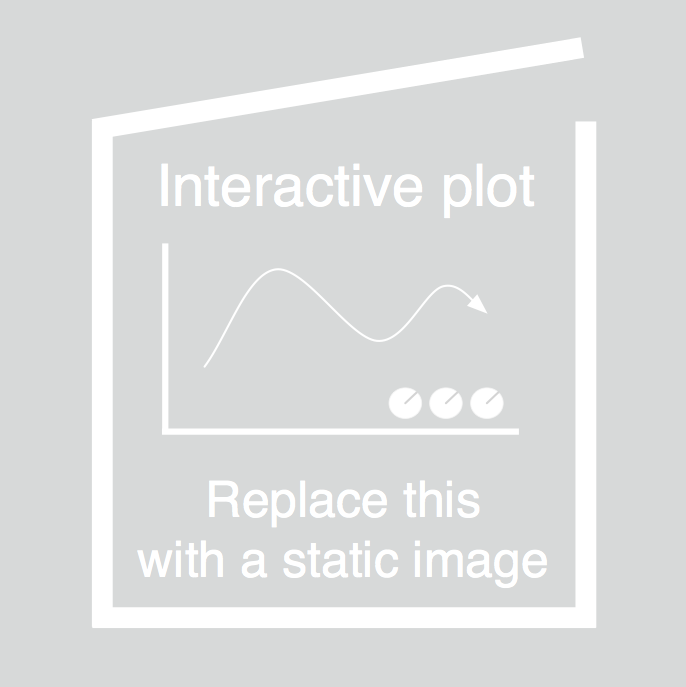
\includegraphics[width=0.70\columnwidth]{./static.png}
\caption{{%
}}
\end{center}
\end{figure}

\section{REFERENCES }\label{references}

Ahmed, T. (2016). \emph{Modeling the renewable energy transition in
Canada: techno-economic assessments for energy management}. Springer.

Alberta Electric System Operator (AESO). (2010). Phase Two Wind
Integration. Working Paper, Market Services Division. Calgary, Alberta.
https://www.aeso.ca/downloads/Phase\_II\_Wind\_Integration\_Recommendation\_-\_Final.pdf.
{[}Accessed Apr 4, 2017.{]}

Bakke, G. A. (2016). \emph{The grid: the fraying wires between Americans
and our energy future}. Bloomsbury USA.

Buysse, J., Fernagut, B., Harmignie, O., de Frahan, B. H., Lauwers, L.,
Polome, P., Van Meensel, J. (2007). Farm-based modelling of the EU sugar
reform: impact on Belgian sugar beet suppliers. \emph{European Review of
Agricultural Economics}, \emph{34}(1), 21--52.

Biggar, D. R., Hesamzadeh, M. R. (2014). \emph{The Economics of
Electricity Markets}. \emph{The Economics of Electricity Markets}.

Behboodi, S., Chassin, D. P., Djilali, N., Crawford, C. (2017).
Interconnection-wide hour-ahead scheduling in the presence of
intermittent renewables and demand response: A surplus maximizing
approach.~\emph{Applied Energy},~189, 336-351.

Benitez, L.E., Benitez, P.C., van Kooten, G.C. (2008). The Economics of
Wind Power with Energy Storage, \emph{Energy Economics} 30(4):
1973-1989.

Castronuovo, E.D., Lopes, J.A.P., (2004). Optimal operation and hydro
storage sizing of a wind-hydro power plant. Electrical Power and Energy
Systems 26, 771--778.

Canadian Wind Energy Association. (2016). Wind energy continues rapid
growth in Canada in 2015. Retrieved from
http://canwea.ca/wind-energy-continues-rapid-growth-in-canada-in-2015/
{[}Accessed April 6, 2017{]}

Chen, X., \& Onal, H. (2012). Modeling Agricultural Supply Response
Using Mathematical Programming and Crop Mixes. \emph{American Journal of
Agricultural Economics}, \emph{94}(3), 674--686.

David Suzuki Foundation. (2016). Coal-fired power worsening health and
climate nation-wide \textbar{} News. Retrieved from
http://www.davidsuzuki.org/media/news/2016/11/coal-fired-power-worsening-health-and-climate-nation-wide/
{[}Accessed April 6, 2017{]}.

EIA, (2010). Updated Capital Cost Estimates for Electricity Generation
Plants. U.S. Energy Information Administration.
http://www.eia.gov/oiaf/beck\_plantcosts/index.html {[}Accessed April 5,
2016{]}.

Environment Canada. (2011). \emph{Canada's Emissions Trends}.
https://doi.org/EN81-18/2013E-PDF {[}Accessed April 5, 2016{]}.

Frew, B., Gallo, G., Brinkman, G., Milligan, M., Clark, K., Bloom, A.
(2016).~\emph{Impact of Market Behavior, Fleet Composition, and
Ancillary Services on Revenue Sufficiency~}(No. NREL/PR-6A20-66384).
NREL (National Renewable Energy Laboratory (NREL), Golden, CO (United
States)).

Government of Alberta, (2015). Climate Leadership Plan will protect
Albertans' health, environment and economy. November 22.
http://www.alberta.ca/release.cfm?xID=
38885E74F7B63-A62D-D1D2-E7BCF6A98D616C09 {[}accessed February 10,
2016{]}.

Government of Canada, (2011). Reduction of Carbon Dioxide Emissions from
Coal-Fired Generation of Electricity Regulations, \emph{Canada Gazette}
Vol. 145, No. 35.

Government of Canada, (2016). \emph{Canada's Second Biennial Report on
Climate Change}. Environment and Climate Change Canada. 52pp.
https://www.ec.gc.ca/GES-GHG/default.asp?lang=En\&n=02D095CB-1
{[}Accessed April 5, 2017{]}.

Guo, G. (2017). \emph{Why Is Asia Returning to Coal?} The Diplomat.
Retrieved from
http://thediplomat.com/2017/02/why-is-asia-returning-to-coal/
{[}Accessed 5 Apr. 2017{]}.

Hallberg, P., Claxton, A., Raedemaeker, P. De, Holm, A., Foosnaes,
Martin, J. G., Mallet, P. (2011). Views on Demand-Side Participation:
Involving Customers, Improving Markets, Enhancing Network Operation, 23.

Hanley, S. (2016). China, Japan, Russia, And South Korea Plan Super Grid
For Renewable Energy -. Retrieved from
http://solarlove.org/china-japan-russia-south-korea-super-grid-renewable/
{[}Accessed April 6, 2017{]}.

Heckelei, T. (2002). Calibration and estimation of programming models
for agricultural supply analysis, University of Bonn Habitation Thesis,
Bonn.

Heckelei, T. and Britz, W. (2000). Positive mathematical programming
with multiple data points, Cahiers d'Economie et Sociologie Rurales 57,
28--50.

Heckelei, T. and Britz, W. (2005). Models based on positive mathematical
programming: state of the art and further extensions, in Arfini, F.
(ed.), Modelling Agricultural Policies: State of the Art and New
Challenges. Proceedings of the 89th European Seminar of the European
Association of Agricultural Economics, University of Parma, Parma, pp.
48--73.

Heckelei, T. and Wolff, H. (2003). Estimation of constrained
optimisation models for argicutural supply analysis based on maximum
entropy, \emph{European Review of Agricultural Economics} 30, 27--50.

Heckelei, T., Britz, W., Zhang, Y. (2012). Positive Mathematical
Programming Approaches -- Recent Developments in Literature and Applied
Modelling. \emph{Bio-Based and Applied Economics}, \emph{1}(1),
109--124.

Henton, D., Varcoe, C. (2015). Early shutdown of coal-fired power plants
could cost billions of dollars:~analyst, \emph{Calgary Herald}, November
25.

Howitt, R. E. (1995). Positive Mathematical Programming. \emph{American
Journal of Agricultural Economics}, \emph{77}(2), 329.

International Energy Agency. (2014). Technology Roadmap Solar
Photovoltaic Energy - 2014 edition. Retrieved from
https://www.iea.org/publications/freepublications/publication/TechnologyRoadmapSolarPhotovoltaicEnergy\_2014edition.pdf
{[}Accessed April 6, 2017{]}.

Joskow, P.L., (2006). Competitive Electricity Markets and Investment in
New Generating Capacity. CEEPR WP 06-009. Center for Energy and
Environmental Policy Research, Department of Economics and Sloan Scholl
of Management, MIT, Cambridge, MA. April 28. 74pp.
http://dspace.mit.edu/bitstream/handle/1721.1/45055/2006-009.pdf?sequence=1
{[}accessed Apr. 4, 2017{]}.

Joskow, P. L. (2008). Capacity payments in imperfect electricity
markets: Need and design. \emph{Utilities Policy}, \emph{16}(3),
159--170.

Joskow, P.L., (2011). Comparing the Costs of Intermittent and
Dispatchable Generating Technologies, \emph{American Economic Review,
Papers and Proceedings} 101(3): 238-241.

Joskow, P. L. (2012). Creating a Smarter U.S. Electricity Grid.
\emph{The Journal of Economic Perspectives} , \emph{26}(1), 29--47.

Lazard. (2016). \emph{Levelized Cost of Storage - Volume 2}.
https://doi.org/10.1080/14693062.2006.9685626 {[}accessed Apr. 4,
2017{]}.

Lazard. (2016). \emph{Lazard's Levelized Cost of Energy Analysis}.
Retrieved from
https://www.lazard.com/media/438038/levelized-cost-of-energy-v100.pdf
{[}accessed Apr. 4, 2017{]}.

Liik, O., Oidram, R., Keel, M., (2003). Estimation of Real Emissions
Reduction caused by Wind Generators. Paper presented at the
International Energy Workshop, 24--26 June. IIASA, Laxenburg, Austria.

Love, M.L. Pitt, Niet, T., McLean, G., (2003). Utility-Scale Energy
Systems: Spatial and Storage Requirements, Working Paper. Institute for
Integrated Energy Systems. University of Victoria, BC.

Lovering, J.R., Yip, A., Nordhaus, T. (2016). Historical Construction
Costs of Global Nuclear Power Reactors, \emph{Energy Policy} 91:
371-382.

Lund, H., (2005). Large-scale integration of wind power into different
energy systems, Energy 30(13): 2402-2412.

Korpaas, M., Holen, A.T., Hildrum, R. (2003). Operation and sizing of
energy storage for wind power plants in a market system. Electrical
Power and Energy Systems 25, 599--606.

Seyboth, K, Sverrisson, F., Appavou, F., Brown, A., Epp, B., Leidreiter,
A., Sovacool, B. (2016). \emph{Renewables 2016 Global Status Report}.
\emph{Global Status Report} .

Maddaloni, J. D., Rowe, A.M., van Kooten, G.C. (2008). Network
constrained wind integration on Vancouver Island, Energy Policy 36(2):
591-602.

McCarthy, S. (2016). Ottawa to phase out coal, aims for virtual
elimination by 2030 - The Globe and Mail. Retrieved from
http://www.theglobeandmail.com/report-on-business/industry-news/energy-and-resources/ottawa-to-announce-coal-phase-out-aims-for-virtual-elimination-by-2030/article32953930/
{[}Accessed April 6, 2017{]}.

Milligan, M., Schwartz, M., Wan, Y., (2003). Statistical Wind Power
Forecasting Models: Results for U.S. Wind Farms. National Renewable
Energy Laboratory, Golden, CO.

Murphy, K., Knaus, C. (2017). South Australian blackout blamed on
thermal and wind generator failures, plus high demand \textbar{}
Australia news \textbar{} The Guardian. Retrieved from
https://www.theguardian.com/australia-news/2017/feb/15/south-australian-blackout-caused-by-demand-and-generator-failures-market-operator-says
{[}Accessed April 4, 2017{]}.

Nolan, J., Parker, D., Van Kooten, G. C., Berger, T. (2009). An overview
of computational modeling in agricultural and resource economics.
\emph{Canadian Journal of Agricultural Economics} , \emph{57}(4),
417--429.

Osborn, L. (n.d.). Sunniest Places in Canada - Current Results.
Retrieved from
https://www.currentresults.com/Weather-Extremes/Canada/sunniest-places.php
{[}Accessed April 6, 2017{]}.

Oswald, J., Raine, M., Ashraf-Ball, H. (2008). Will British weather
provide reliable electricity? Energy Policy 36(8), 3202--3215

Paris, Q., Howitt, R. E. (1998). An Analysis of Ill-Posed Production
Problems Using Maximum Entropy. \emph{American Journal of Agricultural
Economics}, \emph{80}(1), 124--138.

Paris, Q. (2015). PMP and Uniqueness of Calibrating Solution: A
Revision. \emph{SSRN Electronic Journal}.

Payton, M. (2016). Nearly 50 countries vow to use 100\% renewable energy
by 2050. from
http://www.independent.co.uk/news/world/renewable-energy-target-climate-united-nations-climate-change-vulnerable-nations-ethiopia-a7425411.html
{[}Accessed April 06, 2017{]}

Petsakos, A., Rozakis, S. (2015). Calibration of agricultural risk
programming models. \emph{European Journal of Operational Research},
\emph{242} (2), 536--545.

Pitt, L., van Kooten, G.C., Djihali, N. (2005). Utility-Scale Wind
Power: Impacts of Increased Penetration.

Prescott, R., van Kooten, G.C., Zhu, H. (2006). The Potential for Wind
Energy Meeting Electricity Needs on Vancouver Island.

Prescott, R., van Kooten, G.C. (2009). Economic costs of managing of an
electricity grid with increasing wind power penetration with increasing
wind power penetration. \emph{Climate Policy}, \emph{9}(2):155--168.

Ravindran, A., Reklaitis, G.V., Ragsdell, K.M. (2006)~\emph{Engineering
optimization: methods and applications}. John Wiley \& Sons.

Scorah, H., Sopinka, A., van Kooten, G. C. (2012). The economics of
storage, transmission and drought: Integrating variable wind power into
spatially separated electricity grids. \emph{Energy Economics},
\emph{34} (2), 536--541.

Scorah, H. (2010). Integration of Wind Power in Deregulated Power
Systems. \emph{Thesis}.

Sheffield, H. (2016). Solar just made more power than coal in the UK for
the first month ever \textbar{} The Independent. Retrieved from
http://www.independent.co.uk/news/business/news/solar-just-made-more-power-than-coal-in-the-uk-for-the-first-month-ever-a7074621.html
{[}Accessed April 6, 2017{]}.

Stanley, T. D., Doucouliagos, H. (2012). \emph{Meta-regression analysis
in economics and business}. Routledge.

Stoft, S., (2002). \emph{Power System Economics. Designing Markets for
Electricity}. Piscataway, NJ: IEEE Press/Wiley-InterScience.

Timilsina, G.R., van Kooten, G.C., Narbel, P.A., (2013). Global Wind
Power Development: Economics and Policies, \emph{Energy Policy} 61:
642-652.

U.S. Energy Information Administration, (2013). Form EIA-860, Annual
Electric Generator Report. Operable Generating Units in the United
States by State and Energy Source, 2013.
http://www.eia.gov/electricity/data/eia860/index.html {[}Accessed May 5,
2015{]}.

UNEP and Bloomberg, F. S. (2016). Global Trends in Renewable Energy
Investment. Retrieved from
http://fs-unep-centre.org/sites/default/files/publications/globaltrendsinrenewableenergyinvestment2016lowres\_0.pdf
{[}Accessed April 4, 2017{]}

van Kooten, G. C. (2010). Wind power: the economic impact of
intermittency. \emph{Letters in Spatial and Resource Sciences},
\emph{3} (1), 1--17.

van Kooten, G.C. (2012). Climate Change, Climate Science and Economics:
Prospects for a Renewable Energy Future. Dordrecht, NL: Springer.

van Kooten, G. C., Johnston, C., Wong, L. (2013). Wind versus nuclear
options for generating electricity in a carbon-constrained world:
strategizing in an energy-rich economy.~\emph{American Journal of
Agricultural Economics},~\emph{95}(2), 505-511.

Wang, H. (2016).~Economic Mechanisms for Integrating Smart Grid
Technologies into Power Systems~(Doctoral dissertation, The Chinese
University of Hong Kong (Hong Kong)).

\end{document}

